\chapter{Localized Solutions of Nonlinear Harmonic Oscillator with Periodic Pseudopotential}

\section{Objectives}

In this chapter we study localized solutions of Gross--Pitaevskii equation with a harmonic-oscillator (parabolic) trapping potential and a periodic pseudopotential in front of cubic term.
The effective one-dimensional GPE for mean-fields wave function $\Psi(t, x)$ is
\begin{equation}
	i \Psi_t + \Psi_{xx} - \dfrac{1}{2} a^2 x^2 \Psi + P(x) |\Psi|^2 \Psi = 0,
\label{eq:nho}
\end{equation}
where $a^2$ is the strength of the harmonic-oscillator potential, and pseudopotential $P(x)$ is a function of period $L = 2 \pi / \Omega$:
\begin{equation}
	P(x + 2 \pi / \Omega) = P(x).
\end{equation}
Such model can be achieved by means of combination of a magnetic trap and an optical lattice which induces the periodic pseudopotential via the Feshbach resonance \cite{SakaguchiMalomed2010}.
Intervals with positive (negative) values of $P(x)$ correspond to spatial domains with attractive (repulsive) interactions between particles.

The model includes {\it two scales}: the characteristic harmonic-oscillator length $l_{\mathrm{HO}} \sim 1 / \sqrt{a}$, and period $L = 2 \pi / \Omega$ of the pseudopotential.
In particular, the limit case of the wide harmonic-oscillator trap $\Omega \gg 2 \pi \sqrt{a}$, is a physically relevant one.
Let's introduce additional rescaling
\begin{equation}
	t \to \dfrac{a}{\sqrt{2}} t, \quad x \to \dfrac{\sqrt{a}}{\sqrt[4]{2}} x, \quad \Psi \to \dfrac{\sqrt[4]{2}}{\sqrt{a}} \Psi.
\end{equation}
This allows to fix $a \equiv 1$ and convert \eqref{eq:nho} into a normalized form
\begin{equation}
	i \Psi_t + \Psi_{xx} - x^2 \Psi + P(x) |\Psi|^2 \Psi = 0,
\label{eq:nho-scaled}
\end{equation}
where $P(x)$ is periodic with spatial frequency $\widetilde{\Omega} = \Omega / \sqrt{a}$.
In what follows below, symbol $\widetilde{\Omega}$ is replaced by $\Omega$.
To estimate physically relevant values of $\Omega$ we use the results of experimental realization of the periodically-modulated Feshbach resonance in \cite{YamazakiTaieSugawaTakahashi}.
There the corresponding scaled spatial frequency being $\Omega \sim 100$.
It can be made smaller, taking larger $a$.

Equation \eqref{eq:nho-scaled} is our basic model.
The objective of our analysis is to study its localized stationary solutions of the form
\begin{equation}
	\Psi(t, x) = u(x) e^{-i \omega t},
\end{equation}
where real-valued function $u(x)$ satisfies equation
\begin{equation}
	u_{xx} + (\omega - x^2) u + P(x) u^3 = 0
\label{eq:stationary-nho}
\end{equation}
with localization boundary conditions
\begin{equation}
	\lim \limits_{x \to \pm \infty} u(x) = 0.
\end{equation}
During our numerical analysis we focus on the practically important case when the pseudopotential function $P(x)$ in \eqref{eq:nho-scaled} is taken as a sum of constant and harmonic parts of a prototypical cosine form:
\begin{equation}
	P(x) = P_0 + P_1 \cos (\Omega x).
\label{eq:nho-pseudopotential}
\end{equation}

As we say it in Chapter~\ref{chapter:III} stability of solutions is a critically important property.
Linear stability of localized solutions is addressed by considering of small perturbations of a solution $u(x)$ of the form:
\begin{equation}
	\Psi(t, x) = \left( u(x) + (v(x) + w(x)) e^{\lambda t} + (v^{\dagger}(x) - w^{\dagger}(x)) e^{\lambda^{\dagger} t} \right) e^{-i \omega t},
\label{eq:perturabation-nho}
\end{equation}
where $|v(x)| \ll 1$, $|w(x)| \ll 1$.
Substituting \eqref{eq:perturabation-nho} into \eqref{eq:nho-scaled} and performing linearization with respect to $v(x)$ and $w(x)$, we arrive at eigenvalue problem
\begin{equation}
	i
	\begin{pmatrix}
		0 & \mathcal{L}_- \\
		\mathcal{L}_+ & 0
	\end{pmatrix}
	\begin{pmatrix}
		v \\ w
	\end{pmatrix} =
	\lambda
	\begin{pmatrix}
		v \\ w	
	\end{pmatrix},
\label{eq:eigenvalue-problem-nho}
\end{equation}
where 
\begin{eqnarray*}
	&& \mathcal{L}_- = \partial_{xx} + \omega -x^2 + P(x) u^2; \\
	&& \mathcal{L}_+ = \partial_{xx} + \omega -x^2 + 3 P(x) u^2.
\end{eqnarray*}
This problem is similar to the previously considered problem \eqref{eq:eigenvalue-problem}.
Fourier Collocation Method from Chapter~\ref{chapter:III} is also applicable for effective numerical evaluation of spectrum \eqref{eq:eigenvalue-problem-nho}.
Eigenvalues with non-zero real part rise to the instability, while pure imaginary spectrum indicates that solutions is linearly stable.
Again, we note that the eigenvalues appears in pairs and quadruples, i.e. if $\lambda$ is an eigenvalue, then $-\lambda$, $\lambda^{\dagger}$, $-\lambda^{\dagger}$ are eigenvalues too.

For the analytical analysis during this chapter it's convenient to rewrite eigenvalue problem \eqref{eq:eigenvalue-problem-nho} in the equivalent form:
\begin{equation}
	\mathcal{L}_+ \mathcal{L}_- w = \Lambda w, \quad \Lambda = -\lambda^2.
\label{eq:eigenvalue-problem-nho-analytical}
\end{equation}
In terms of \eqref{eq:eigenvalue-problem-nho-analytical}, a solution $u(x)$ passes the linear stability test if the spectrum of eigenvalues $\Lambda$ is all-real positive.

\subsection{Solutions with linear counterpart}

An important class of localized solutions of equation \eqref{eq:stationary-nho} is {\it nonlinear solutions with linear counterpart}.
Such terminology has been adopted in \cite{AgostaMalomedPresilla, AgostaPresilla}.
Existence of such solution came from the consideration of the low-amplitude limit.
% TODO: Add reference to the definition of norm from the overall introduction, not from Chapter III.
For a small value of norm $N$, see \eqref{eq:norm}, the nonlinear term in \eqref{eq:stationary-nho} may be neglected, which leads to the ordinary harmonic-oscillator equation
\begin{equation}
	u_{xx} + (\omega - x^2) u = 0.
\label{eq:ho}
\end{equation}
Equation \eqref{eq:ho} produces the commonly known set of eigenvalues and eigenfunctions:
\begin{equation}
	\tilde{\omega}_n = 2n + 1; \quad \tilde{u}_n(x) = \dfrac{1}{\sqrt{2^n n! \sqrt{\pi}}} H_n(x) e^{-\frac{-1}{2} x^2}; \quad n = 0, 1, \dots,
\label{eq:ho-solutions}
\end{equation}
where $H_n(x)$ functions are Hermite polynomials.
In particular,
\begin{equation*}
	H_0(x) = 1, \quad H_1(x) = 2x, \quad H_2(x) = 4x^2 - 2.	
\end{equation*}

When the nonlinearity is switched on, each linear eigenstate $(\tilde{\omega}_n, \tilde{u}_n(x))$ bifurcates into a one-parameter set $\Gamma_n = (\omega_n, u_n(x))$ of small-amplitude localized solutions of \eqref{eq:stationary-nho}.
These solutions are produced by equation \eqref{eq:stationary-nho} and become essentially nonlinear with the increase of $N$ and distance between $\omega_n$ and $\tilde{\omega}_n$.
Localized solutions from family $\Gamma_n$ feature the same parity as the corresponding linear eigenfunction $\tilde{u}_n(x)$, solution with even $n$ are even functions of $x$, and those with the odd $n$ are odd.
Localized solution with $n = 0$ originates form the ground state of the harmonic-oscillator.

During our analysis it's interesting to compare the results with the well-studied case of Gross--Pitaevskii equation \eqref{eq:nho-scaled} with constant $P(x)$ (negative or positive).
In this case $P_1 \equiv 0$ in \eqref{eq:nho-pseudopotential} and equation \eqref{eq:stationary-nho} takes form
\begin{equation}
	u_{xx} + (\omega - x^2) u + P_0 u^3 = 0.
\label{eq:nho-constant}
\end{equation}
Let's call \eqref{eq:nho-constant} the {\it nonlinear harmonic-oscillator} equation with constant pseudopotential.
The case $P_0 > 0$ ($P_0 < 0$) corresponds to the attractive (repulsive) interparticle interactions.
It's convenient to illustrate branches of localized solutions of equation \eqref{eq:nho-constant} by means of respective $N(\omega)$ curves, which are presented in Figure~\ref{fig:branches-constant-nho}, as per \cite{ZezyulinAlfimovKonotopPerecGarcia2007, ZezyulinAlfimovKonotopPerecGarcia2008} for the cases $P_0 = \pm 1$.
The branches $\Gamma_n$, $n = 0, 1, \dots$, correspond to the solutions with linear counterparts, bifurcating from them at the points $\tilde{\omega}_n = 2n + 1$, $N = 0$.
All the branches being represented by monotonous functions $N(\omega)$.
Other results obtained for localized solutions of \eqref{eq:nho-constant} can be presented as follows.
\begin{itemize}
	\item Presumably, there exist no nonlinear solutions of \eqref{eq:nho-constant} without linear counterpart \cite{AlfimovZezyulin}.
	\item Solutions corresponding to families $\Gamma_0$, $\Gamma_1$ are stable in the small-amplitude limit and for moderate and large amplitudes as well for both signs of $P_0$.
	\item
		The small-amplitude solutions belonging to the branch $\Gamma_2$ are unstable.
		For the case $P_0 > 0$, the instability of the branch $\Gamma_2$ persists for $\omega^* < \omega < 5$, where $\omega^* \approx 3.83$.
		According to the numerical study at $\omega < \omega^*$ these solutions was reported to be stable \cite{AlfimovZezyulin}.
		For the case $P_0 < 0$ the branch $\Gamma_2$ is fully unstable. 
\end{itemize}

\begin{figure}[h]
\centering
	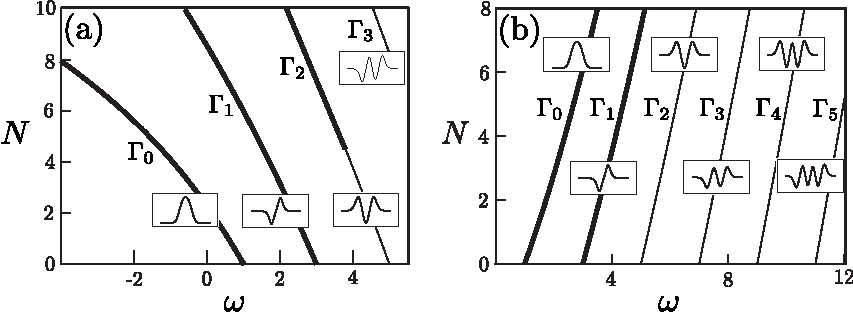
\includegraphics[scale = 1]{pic/stability for nho with constant pseudopotential}
	\caption{
		$N(\omega)$ curves for equation \eqref{eq:nho-constant}, with (a) $P_0 = 1$, (b) $P_0 = -1$.
		Bold (thin) segments correspond to stable (unstable) solutions.
		Insets show schematic profiles of solutions $u_n(x)$ from each family $\Gamma_n$.
	}
\label{fig:branches-constant-nho}
\end{figure}

Before we can move on let's briefly resume our goals in this chapter.
We study localized solutions of equation \eqref{eq:nho-scaled} with periodic pseudopotential \eqref{eq:nho-pseudopotential}.
We apply linear stability analysis to find stable solutions among them.
Our baseline model for comparison is well-studied equation \eqref{eq:nho-constant} for nonlinear harmonic-oscillator with constant pseudopotential.
We pay special attention to the localized solutions with linear counterpart, and study how the presence of periodic pseudopotential $P(x)$ of the cosine form \eqref{eq:nho-pseudopotential} affects their stability.

\section{Small-Amplitude Localized Solutions with Linear Counterpart}

For Eq.~\eqref{eq:nho-scaled} let's consider a small-amplitude limit of solutions with linear counterpart.
As we say above, such solutions $u_n(x)$ originate from the bifurcation of eigenstates $(\tilde{\omega}_n, \tilde{u}_n(x))$ of harmonic-oscillator equation \eqref{eq:ho} and form families $\Gamma_n = (\omega_n, u_n(x))$.
If the amplitude of $u_n(x)$ is small the localized solutions from branch $\Gamma_n$ are approximated by expansions \cite{ZezyulinAlfimovKonotopPerecGarcia2008},
\begin{equation}
	u_n(x) = \varepsilon \tilde{u}_n(x) + o(\varepsilon), \quad \omega_n = \tilde{\omega}_n - \varepsilon^2 \Delta_n + o(\varepsilon^2),
\label{eq:small-amplitude-expansion}
\end{equation}
where $\varepsilon \ll 1$ is a small parameter, and
\begin{equation}
	\Delta_n = \int \limits_{-\infty}^{+\infty} P(x) \tilde{u}_n^4(x) dx = \dfrac{1}{2^{2n} (n!)^2 \pi} \int \limits_{-\infty}^{+\infty} P(x) H_n^4(x) e^{-2x^2} dx.
\end{equation}

Let's address stability of these small-amplitude solutions.
We note that with the help of expansion \eqref{eq:small-amplitude-expansion}, operator $\mathcal{L}_+ \mathcal{L}_-$ in \eqref{eq:eigenvalue-problem-nho-analytical} may be considered as a perturbation of operator $\mathcal{L}_n^2$, where
\begin{equation}
	\mathcal{L}_n = \partial_{xx} + 2n + 1 - x^2.
\end{equation}
Specifically,
\begin{eqnarray*}
	&& \mathcal{L}_+ = \mathcal{L}_n + \varepsilon^2 (3 P(x) \tilde{u}_n^2(x) - \Delta_n) + o(\varepsilon^2); \\
	&& \mathcal{L}_- = \mathcal{L}_n + \varepsilon^2 (P(x) \tilde{u}_n^2(x) - \Delta_n) + o(\varepsilon^2).
\end{eqnarray*}
% TODO: Consider to use $\mathcal{M}_n$ instead of $M_n$.
So, for the operator $\mathcal{L}_+ \mathcal{L}_-$ we can write
\begin{equation}
	\mathcal{L}_+ \mathcal{L}_- = \mathcal{L}_n^2 + \varepsilon^2 M_n + o(\varepsilon^2),
\label{eq:perturbed-operator}
\end{equation}
where
\begin{equation}
	M_n = (2 P(x) \tilde{u}_n^2(x) - \Delta_n) \mathcal{L}_n + \mathcal{L}_n (P(x) \tilde{u}_n^2(x) - \Delta_n).
\label{eq:Mn}
\end{equation}
Operator $\mathcal{L}_n$ is self-adjoint in $L^2$ space, and its spectrum consists of eigenvalues $\varkappa_k = 2(n - k)$ with corresponding eigenfunctions $\tilde{u}_k(x)$, $k = 0, 1, \dots$  in the form \eqref{eq:ho-solutions}.
The spectrum is equidistant, all the eigenvalues being simple.
There are infinitely many negative eigenvalues, $n$ positive eigenvalues, and one zero eigenvalue.
The eigenvalues $\widetilde{\Lambda}_k$ of operator $\mathcal{L}_n^2$ are squared eigenvalues of $\mathcal{L}_n$, i.e. $\widetilde{\Lambda}_k = \varkappa_k^2 = 4 (k - n)^2$, corresponding to the same eigenfunctions $\tilde{u}_k(x)$.
This means that the spectrum of $\mathcal{L}_n^2$ includes $n$ {\it double positive eigenvalues} $\widetilde{\Lambda}_k = 4 (n - k)^2$, $k = 0, 1, \dots, (n - 1)$, one {\it simple zero eigenvalue} and {\it infinitely many simple positive eigenvalues}.
Each of the double eigenvalues has an invariant subspace spanned by two functions, $\tilde{u}_k(x)$ and $\tilde{u}_{2n - k}(x)$.
If $n = 0$, then all eigenvalues of $\mathcal{L}_n^2$ are simple.

Generically, small perturbation of $\mathcal{L}_n$ results in {\it splitting} of the double eigenvalues.
Each of them can split into (i) two real eigenvalues of the perturbed operator or (ii) two complex-conjugate eigenvalues.
If the case (i) takes place for each double eigenvalue, then small-amplitude localized solutions bifurcating form the $n$-th linear eigenstate are marginally stable, at least in some vicinity of the bifurcation.
However, if at least for one double eigenvalue the case (ii) takes place, then the bifurcating small-amplitude solutions  are unstable in vicinity of the bifurcation.

To address the splitting of double eigenvalues when passing from operator $\mathcal{L}_n^2$ to the perturbed one, $\mathcal{L}_+ \mathcal{L}_-$ in \eqref{eq:perturbed-operator}, we construct an {\it asymptotic expansion for perturbed eigenvalues} following \cite{ZezyulinAlfimovKonotopPerecGarcia2008}.
Under the actions of the perturbation, each double eigenvalue $\widetilde{\Lambda}_k$ splits into two simple ones:
\begin{equation}
	\Lambda_{k, 1} = \widetilde{\Lambda}_k + \varepsilon^2 \gamma_1 + o(\varepsilon^2), \quad \Lambda_{k, 2} = \widetilde{\Lambda}_k + \varepsilon^2 \gamma_2 + o(\varepsilon^2),
\end{equation}
where the coefficients $\gamma_{1,2}$ are the eigenvalues of the 2$\times$2 matrix
\begin{equation}
	\widetilde{M}_n =
	\begin{pmatrix}
		\langle M_n \tilde{u}_k, \tilde{u}_k \rangle & \langle M_n \tilde{u}_k, \tilde{u}_{2n - k} \rangle \\
		\langle M_n \tilde{u}_{2n - k}, \tilde{u}_k \rangle & \langle M_n \tilde{u}_{2n - k}, \tilde{u}_{2n - k} \rangle
	\end{pmatrix}.
\end{equation}
Therefore, if the eigenvalues of $\widetilde{M}_n$ are real for each $k = 0, 1, \dots, n - 1$, then the spectrum of $\mathcal{L}_+ \mathcal{L}_-$ remains real and the nonlinear localized solution $u_n(x)$ is stable, at least for sufficiently small $\varepsilon$.
Otherwise, if eigenvalues of $\widetilde{M}_n$ are complex for some $k = 0, 1, \dots, n - 1$, then solution $u_n(x)$ is unstable in a vicinity of the bifurcation.
None that, as no double eigenvalues exist for $n = 0$, the small-amplitude solutions of the family $\Gamma_0$ are stable for any $P(x)$.

Using explicit expressions for the eigenfunctions $\tilde{u}_n(x)$ from \eqref{eq:small-amplitude-expansion} and expressions for $M_n$ from \eqref{eq:Mn}, one can compute the entries of the matrix $\widetilde{M}_n$:
\begin{align}
\langle M_n \tilde{u}_k &, \tilde{u}_k \rangle = \frac{8(n-k)}{\pi 2^{(n+k)} n! k!} \int \limits_{-\infty }^{+\infty} P(x) H_n^2(x) H_k^2(x) e^{-2 x^2} dx \notag \\ & - \frac{4(n-k)}{\pi 2^{2n}(n!)^2} \int \limits_{-\infty }^{+\infty} P(x) H_n^4(x) e^{-2 x^2} dx; \label{eq:Mn11} \\
\langle M_n \tilde{u}_k &, \tilde{u}_{2n-k} \rangle = -\langle M_n \tilde{u}_{2n-k}, \tilde{u}_k \rangle = \notag \\ & = \frac{4 (n-k)}{\pi 2^{2n} n! \sqrt{k! (2n-k)!}} \int \limits_{-\infty}^{+\infty} P(x) H_n^2(x) H_{2n-k}(x) H_k(x) e^{-2 x^2} dx;  \label{eq:Mn12} \\
\langle M_n \tilde{u}_{2n-k} &, \tilde{u}_{2n-k} \rangle = -\frac{8(n-k)}{\pi 2^{(3n-k)} n! (2n-k)!} \int \limits_{-\infty}^{+\infty} P(x) H_n^2(x) H_{2n-k}^2(x) e^{-2 x^2} dx \notag \\ & + \frac{4(n-k)}{\pi 2^{2n} (n!)^2} \int \limits_{-\infty}^{\infty} P(x) H_n^4(x) e^{-2 x^2} dx. \label{eq:Mn22}
\end{align}
Formulas \eqref{eq:Mn11} -- \eqref{eq:Mn22} with $P(x) = \pm 1$ were used in \cite{ZezyulinAlfimovKonotopPerecGarcia2008} to explore the stability of small-amplitude nonlinear solutions in the model with constant pseudopotential.

\section{Branches of Nonlinear Localized Solutions for Periodic Pseudopotential, $P(x) = P_0 + P_1 \cos (\Omega x)$}

We present our numerical and analytical results for pseudopotential of the cosine form \eqref{eq:nho-pseudopotential}.
It represents a sum of a constant part $P_0$ and a periodic part $P_1 \cos (\Omega x)$.
In what follow below we conclude that the relation between the magnitudes of $|P_0|$ and $|P_1|$ is important.
Hence, it's necessary to consider two cases separately: (a) $|P_0| \gtrsim |P_1|$, when the constant component is not negligible, and (b) $|P_0| \ll |P_1|$, when the constant component is negligible and pseudopotential \eqref{eq:nho-pseudopotential} should be treated as a function with zero mean. 
We consider each of these cases separately.

\subsection{Periodic pseudopotential with Non-Zero Mean, $|P_0| \gtrsim |P_1|$}

If $P_0$ component of pseudopotential is not negligible, one can scale out the absolute value of it, by replacing 
\begin{equation}
	\Psi \to \Psi / \sqrt{|P_0|}, \quad P_1 / |P_0| \to P_1.
\end{equation}
Equation \eqref{eq:nho-scaled} takes form
\begin{equation}
	i \Psi_t + \Psi_{xx} + x^2 \Psi + (\sigma_0 + P_1 \cos (\Omega x)) |\Psi|^2 \Psi = 0.
\label{eq:nho-non-zero-mean}
\end{equation}
where $\sigma_0 \equiv P_0 / |P_0| = \mathrm{sign} (P_0)$.
Stationary states equation in this case has form
\begin{equation}
	u_{xx} + (\omega - x^2) u + (\sigma_0 + P_1 \cos (\Omega x)) u^3 = 0.
\label{eq:stationary-nho-non-zero-mean}
\end{equation}
A generic picture of localized solutions of equation \eqref{eq:stationary-nho-non-zero-mean} can be obtained by means of a numerical shooting algorithm.
A representative example of the respective $N(\omega)$ curves with $\sigma_0 = 1$, $P_1 = 2$ (which implies that the sign of the pseudopotential periodically flips), and $\Omega = 12$ is displayed in Figure~\ref{fig:branches-cosine-nho-attractive}.
One can immediately observe that, apart from branches $\Gamma_n$ originating from their linear counterparts, numerous branches of localized solutions {\it without linear counterpart} exist too.
Thus, the presence of the periodic component in the pseudopotential essentially enriches the diversity of available solutions.
This contrasts with the case of nonlinear harmonic-oscillator with constant pseudopotential, see Figure~\ref{fig:branches-constant-nho}.
However, we did not find stable solutions without linear counterpart.
On Figure~\ref{fig:branches-cosine-nho-attractive} only stables solutions correspond to branches $\Gamma_0$, $\Gamma_1$, $\Gamma_2$.

\begin{figure}[h]
\centering
	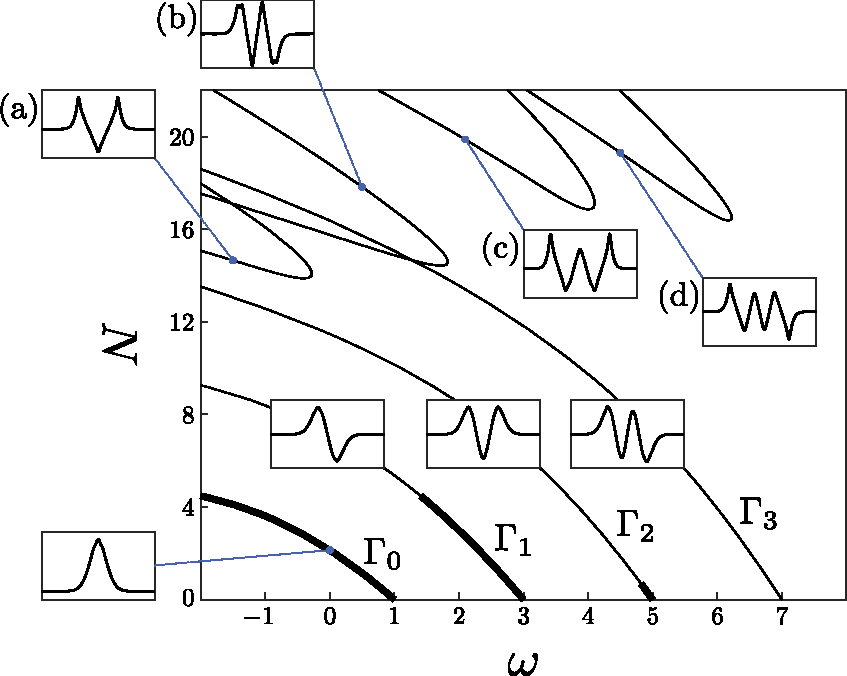
\includegraphics[scale = 1]{pic/branches for cosine nho, case (a)}
	\caption{
		Curves $N(\omega)$ of solution families for equation \eqref{eq:stationary-nho-non-zero-mean} with non-zero mean cosine pseudopotential with $\sigma_0 = 1$, $P_1 = 2$, and $\Omega = 12$.
		This and bold lines show unstable and stable solution families.
		Branches $\Gamma_n$, $n = 0, 1, 2, 3$ represent solutions with linear counterpart.
		Insets on top of branches are representative profiles $u(x)$ of solutions obtained from those families.
		Branches (a), (b), (c), and (d) represent solutions without linear counterpart.
		All of them were found to be unstable.
	}
\label{fig:branches-cosine-nho-attractive}
\end{figure}

\subsection{Periodic pseudopotential with Zero Mean, $|P_0| \ll |P_1|$}

If $P_0$ component of the pseudopotential can be neglected, we drop $P_0$, and rescale equation \eqref{eq:nho-scaled} by replacing
\begin{equation}
	\Psi \to \Psi / \sqrt{|P_1|},
\end{equation}
which leads to the equation
\begin{equation}
	i \Psi_t + \Psi_{xx} + x^2 \Psi - \sigma_1 \cos (\Omega x) |\Psi|^2 \Psi = 0,
\label{eq:stationary-nho-zero-mean}
\end{equation}
where $\sigma_1 = P_1 / |P_1| = \mathrm{sign}(P_1)$.

\section{Summary}

In this chapter we ...
Our main finding can be summarized as follows.